\documentclass[12pt,a4paper]{article}\usepackage[]{graphicx}\usepackage[]{xcolor}
% maxwidth is the original width if it is less than linewidth
% otherwise use linewidth (to make sure the graphics do not exceed the margin)
\makeatletter
\def\maxwidth{ %
  \ifdim\Gin@nat@width>\linewidth
    \linewidth
  \else
    \Gin@nat@width
  \fi
}
\makeatother

\definecolor{fgcolor}{rgb}{0.345, 0.345, 0.345}
\newcommand{\hlnum}[1]{\textcolor[rgb]{0.686,0.059,0.569}{#1}}%
\newcommand{\hlstr}[1]{\textcolor[rgb]{0.192,0.494,0.8}{#1}}%
\newcommand{\hlcom}[1]{\textcolor[rgb]{0.678,0.584,0.686}{\textit{#1}}}%
\newcommand{\hlopt}[1]{\textcolor[rgb]{0,0,0}{#1}}%
\newcommand{\hlstd}[1]{\textcolor[rgb]{0.345,0.345,0.345}{#1}}%
\newcommand{\hlkwa}[1]{\textcolor[rgb]{0.161,0.373,0.58}{\textbf{#1}}}%
\newcommand{\hlkwb}[1]{\textcolor[rgb]{0.69,0.353,0.396}{#1}}%
\newcommand{\hlkwc}[1]{\textcolor[rgb]{0.333,0.667,0.333}{#1}}%
\newcommand{\hlkwd}[1]{\textcolor[rgb]{0.737,0.353,0.396}{\textbf{#1}}}%
\let\hlipl\hlkwb

\usepackage{framed}
\makeatletter
\newenvironment{kframe}{%
 \def\at@end@of@kframe{}%
 \ifinner\ifhmode%
  \def\at@end@of@kframe{\end{minipage}}%
  \begin{minipage}{\columnwidth}%
 \fi\fi%
 \def\FrameCommand##1{\hskip\@totalleftmargin \hskip-\fboxsep
 \colorbox{shadecolor}{##1}\hskip-\fboxsep
     % There is no \\@totalrightmargin, so:
     \hskip-\linewidth \hskip-\@totalleftmargin \hskip\columnwidth}%
 \MakeFramed {\advance\hsize-\width
   \@totalleftmargin\z@ \linewidth\hsize
   \@setminipage}}%
 {\par\unskip\endMakeFramed%
 \at@end@of@kframe}
\makeatother

\definecolor{shadecolor}{rgb}{.97, .97, .97}
\definecolor{messagecolor}{rgb}{0, 0, 0}
\definecolor{warningcolor}{rgb}{1, 0, 1}
\definecolor{errorcolor}{rgb}{1, 0, 0}
\newenvironment{knitrout}{}{} % an empty environment to be redefined in TeX

\usepackage{alltt}
    \setlength\parindent{0pt}
    \usepackage{geometry}
    \usepackage{graphicx}
    \usepackage{grffile}
    \geometry{margin=0.5in}
\IfFileExists{upquote.sty}{\usepackage{upquote}}{}
\begin{document}

    \section*{Octopus}


    Species: \emph{Octopus vulgaris}, Stock code: 1-Western Coast 2-Bottom Trawl

Region: Iberia

Marine Ecoregion: Portugal

Reconstructed catch data used from years 1995 - 2022 

 For figure captions and method see http://www.seaaroundus.org/cmsy-method

    \begin{figure}[ht]
    \centering
    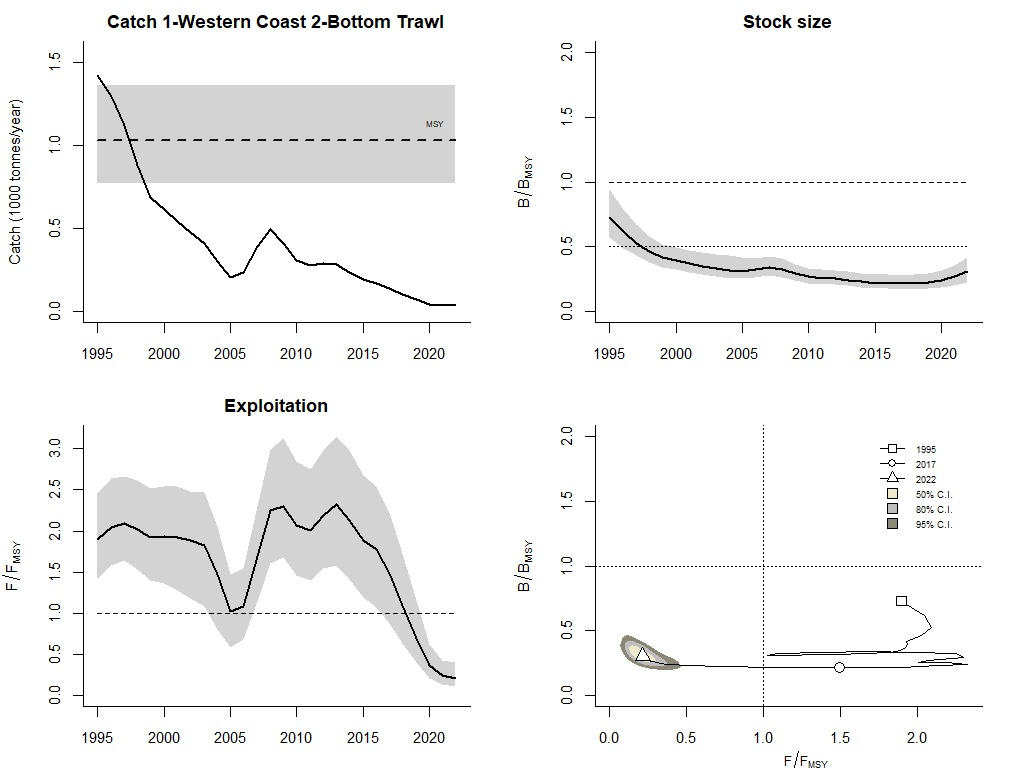
\includegraphics[width=1.00\textwidth ext=.jpg type=jpg]{1-Western Coast 2-Bottom Trawl_MAN.jpg}
    \end{figure}

    \textbf{Results for management (based on BSM analysis)}\\

Fmsy = 0.223, 95\% CL = 0.156 - 0.317 (if B $>$ 1/2 Bmsy then Fmsy = 0.5 r)

Fmsy = 0.138, 95\% CL = 0.0965 - 0.195 (r and Fmsy are linearly reduced if B $<$ 1/2 Bmsy)

MSY = 1.03,  95\% CL = 0.77 - 1.36; Bmsy = 4.6,  95\% CL = 3.27 - 6.65 (1000 tonnes)

Biomass in last year = 1.43, 95\% CL = 0.928 - 2.12 (1000 tonnes)

B/Bmsy in last year = 0.309, 95\% CL = 0.225 - 0.415

Fishing mortality in last year = 0.0291, 95\% CL =0.018 - 0.049

F/Fmsy  = 0.212, 95\% CL = 0.114 - 0.41 

 Comment:  

    \pagebreak

    \begin{figure}[ht]
    \centering
    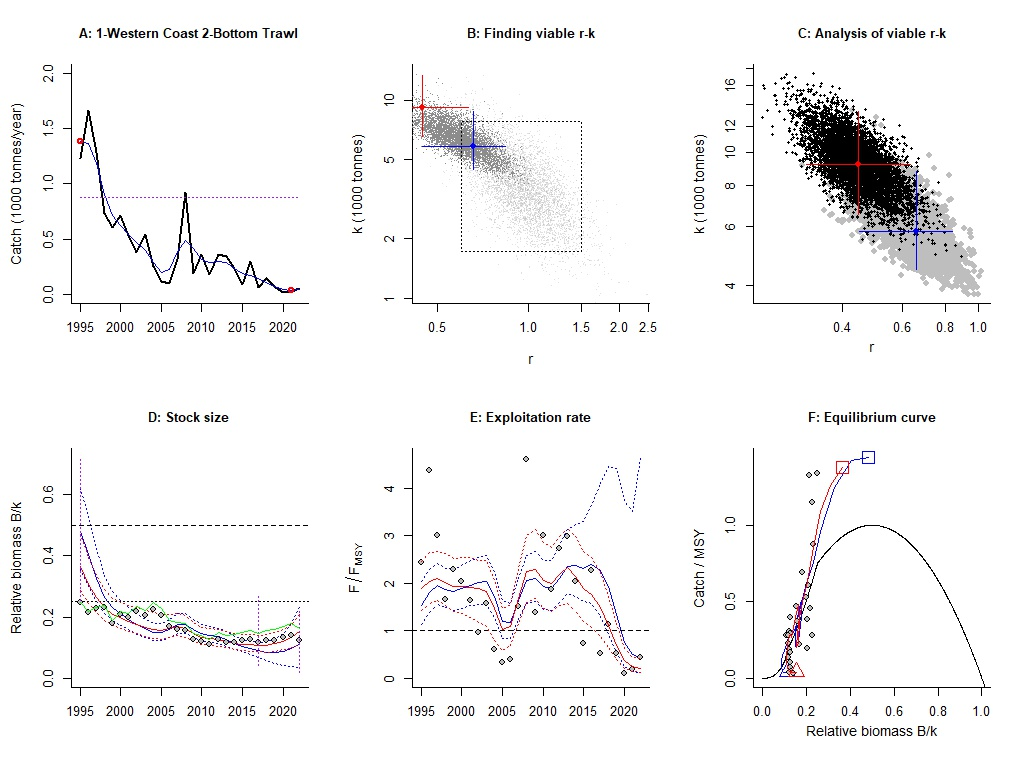
\includegraphics[width=1.00\textwidth ext=.jpg type=jpg]{1-Western Coast 2-Bottom Trawl_AN.jpg}
    \end{figure}

    \textbf{Results of CMSY analysis conducted in JAGS}\\

r = 0.658, 95\% CL = 0.448 - 0.839; k = 5.82, 95\% CL = 4.46 - 8.77 (1000 tonnes)

MSY = 0.957, 95\% CL = 0.751 - 1.24 (1000 tonnes/year)

Relative biomass last year = 0.112 k, 95\% CL = 0.0352 - 0.233

Exploitation F/(r/2) in last year = 0.507 \\

\textbf{Results from Bayesian Schaefer model using catch and CPUE}\\

r = 0.446, 95\% CL = 0.312 - 0.633; k = 9.21, 95\% CL = 6.54 - 13.3

r-k log correlation = -0.672

MSY = 1.03, 95\% CL = 0.77 - 1.36 (1000 tonnes/year)

Relative biomass in last year = 0.112 k, 95\% CL = 0.0352 - 0.233

Exploitation F/(r/2) in last year = 0.237

q = 3.72, 95\% CL = 2.59 - 5.23

Prior range of q = 1.03 - 18.6

Relative abundance data type = CPUE

Prior initial relative biomass = 0.256 - 0.721 default

Prior intermediate relative biomass = 0.0426 - 0.269 in year 2017 default

Prior final relative biomass = 0.0196 - 0.22, default

Prior range for r = 0.6 - 1.5 default, prior range for k = 1.74 - 7.82 (1000 tonnes) default

Source for relative biomass: 

DGRM

    \end{document}
